\chapter{Análisis del problema}\label{cap:analisis}\label{cap:requisitos}\label{ap:req-detallados}

Este capítulo recoge el análisis de requisitos del proyecto. Presenta los actores del
sistema, el modelo de dominio que sostiene los requisitos de información, los requisitos
funcionales y no funcionales, las reglas de negocio, los casos de uso y la matriz de
trazabilidad que enlaza cada requisito con su evidencia. Los
requisitos se identifican con códigos estables tomados de \texttt{.planning/REQUIREMENTS.md},
de modo que la matriz de trazabilidad de este capítulo y la del repositorio coinciden. Los
requisitos abarcan por igual las dos caras del trabajo: la plataforma de catalogación y la
evaluación de recomendadores que se apoya en ella.

\section{Actores del sistema}\label{sec:req-actores}

El sistema distingue dos actores, que enumera la Tabla~\ref{tab:actores}. Para que el tribunal
pueda recorrer el sistema sin registrarse, el entorno incluye una cuenta de usuario ya
preparada, que es una cuenta normal con sus datos y no un actor distinto.

\begin{table}[H]
\centering
\begin{tabularx}{\textwidth}{ | L{0.20\textwidth} | Y | }
    \hline
    \textbf{Actor} & \textbf{Descripción} \\
    \hline
    Visitante & Persona no autenticada que consulta el catálogo, la ficha de un juego y la recomendación por popularidad, y que puede registrarse. \\
    \hline
    Persona usuaria & Titular de una cuenta registrada que inicia sesión y gestiona su lista de pendientes, valora juegos, inventaría copias y se relaciona con sus amigos. \\
    \hline
\end{tabularx}
\caption{Actores del sistema.}
\label{tab:actores}
\end{table}

\section{Requisitos de información: modelo de dominio}\label{sec:req-informacion}

El modelo de dominio distingue tres áreas: el catálogo, la biblioteca personal y las cuentas.
La Figura~\ref{fig:modelo-dominio} las representa junto con las tablas del laboratorio de
evaluación, que describe la Sección~\ref{sec:dis-laboratorio}; los párrafos siguientes
describen las entidades de las tres primeras.

\begin{figure}[H]
    \centering
    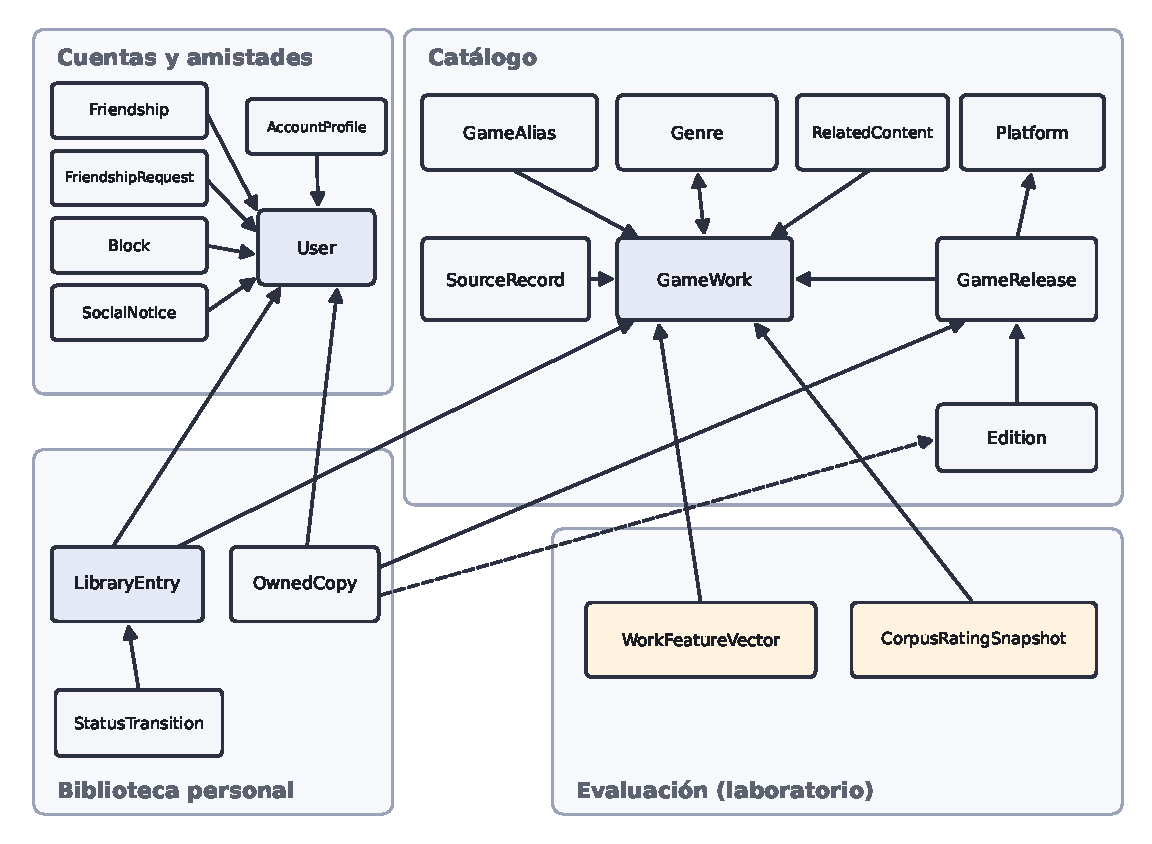
\includegraphics[width=0.95\textwidth]{figures/modelo-dominio.pdf}
    \caption{Modelo de dominio de SavePoint, agrupado por catálogo, biblioteca personal, cuentas y amistades, y laboratorio de evaluación. Cada flecha parte de la entidad que contiene la clave foránea y apunta a la entidad que referencia; la flecha de doble punta indica una relación de muchos a muchos y la discontinua, una referencia opcional. De las copias en propiedad solo se dibujan sus referencias a la versión de lanzamiento y a la edición; \texttt{IgdbImportRun} y \texttt{AssetAttribution} se omiten de la figura y se describen en el texto.}
    \label{fig:modelo-dominio}
\end{figure}

En el catálogo, la entidad central es la obra (\texttt{GameWork}), la identidad canónica de
un título de videojuego con independencia de la plataforma y de la edición. Cada obra puede tener varias publicaciones (\texttt{GameRelease}), una por plataforma
(\texttt{Platform}). Cada publicación puede tener a su vez varias ediciones
(\texttt{Edition}). Los géneros (\texttt{Genre}) se
asocian a la obra mediante una relación de muchos a muchos. Los alias bilingües
(\texttt{GameAlias}) sostienen la búsqueda tolerante. El contenido relacionado (\texttt{RelatedContent}) enlaza
contenido descargable (DLC) y expansiones con su obra padre. La
procedencia de cada obra vive en \texttt{SourceRecord}, con la fuente, el identificador de
origen, la licencia, la fecha de recuperación y un hash del contenido normalizado. La
atribución de cada portada revisada individualmente vive en \texttt{AssetAttribution}, cuya
marca de portada permitida está a falso por defecto. El progreso de una importación de IGDB
se registra en \texttt{IgdbImportRun}, con el cursor de identificador y el estado.

En la biblioteca personal, la entrada de biblioteca (\texttt{LibraryEntry}) representa la
relación entre una persona usuaria y una obra, con su estado en la lista de pendientes y su
valoración. El historial de
transiciones de estado (\texttt{StatusTransition}) es un registro de solo anexado. Las copias
en propiedad (\texttt{OwnedCopy}) representan cada ejemplar, físico o digital, con su formato,
su publicación y su edición.

En las cuentas, el proyecto usa directamente el modelo de usuario de Django
(\texttt{User}), al que se asocian la biblioteca personal y las relaciones de amistad. Las solicitudes (\texttt{FriendshipRequest}), las amistades aceptadas (\texttt{Friendship}) y los bloqueos (\texttt{Block}) son entidades que referencian a dos usuarios. El perfil editable (\texttt{AccountProfile}) guarda el nombre completo, la biografía, la foto, la portada y los ajustes de privacidad, y las notificaciones (\texttt{SocialNotice}) avisan de las solicitudes aceptadas y de las recomendaciones añadidas a pendientes.

La Tabla~\ref{tab:req-informacion} enlaza cada área del modelo con los requisitos de
información que satisface.

\begin{table}[H]
\centering
\begin{tabularx}{\textwidth}{ | L{0.16\textwidth} | Y | C{0.16\textwidth} | }
    \hline
    \textbf{Área} & \textbf{Requisito de información} & \textbf{Códigos} \\
    \hline
    Catálogo & Identidad canónica independiente del proveedor de enriquecimiento. & CAT-04 \\
    \hline
    Catálogo & Registro de fuente, licencia, fecha de recuperación y hash por obra. & DATA-02 \\
    \hline
    Catálogo & Metadatos de plataforma, género, edición y fechas de fuentes aprobadas. & CAT-05 \\
    \hline
    Biblioteca & Estado de la lista de pendientes por persona y obra. & LIB-01 \\
    \hline
    Biblioteca & Valoración con escala consistente. & LIB-02 \\
    \hline
    Biblioteca & Copias en propiedad con formato, plataforma y edición. & INV-01, INV-02 \\
    \hline
    Cuentas & Relaciones de amistad y bloqueo entre personas usuarias. & SOCIAL-03 \\
    \hline
\end{tabularx}
\caption{Áreas del modelo de dominio y requisitos de información asociados.}
\label{tab:req-informacion}
\end{table}

\section{Requisitos funcionales y casos de uso}\label{sec:req-funcionales}\label{sec:req-casos-uso}

La Tabla~\ref{tab:req-funcionales} recoge los requisitos funcionales considerados en el
análisis, con su estado real. Los marcados como completos tienen evidencia en las firmas de
aceptación.

\begin{table}[htp]
\centering
\tablecompact
\begin{tabularx}{\textwidth}{ | L{0.18\textwidth} | Y | C{0.22\textwidth} | }
    \hline
    \textbf{Código} & \textbf{Requisito funcional} & \textbf{Estado} \\
    \hline
    AUTH-01 & Iniciar y cerrar sesión en una cuenta controlada. & Completo \\
    \hline
    PROF-01 & Editar el perfil (nombre, foto, portada, favoritos) y su visibilidad. & Completo \\
    \hline
    SOCIAL-03 & Buscar a otra persona por su alias exacto y gestionar solicitudes de amistad, amistades y bloqueos. & Completo \\
    \hline
    SOCIAL-04 & Consultar la colección, las listas y los comentarios de un amigo aceptado; quien no es amigo solo ve el nombre de usuario. & Completo \\
    \hline
    SOCIAL-05 & Recomendar juegos a un amigo y responder a las recibidas. & Completo \\
    \hline
    CAT-01 & Buscar videojuegos por título. & Completo \\
    \hline
    CAT-02 & Filtrar y ordenar el catálogo por metadatos disponibles. & Completo \\
    \hline
    CAT-03 & Ficha de detalle de cada juego con sus datos y su procedencia. & Completo \\
    \hline
    CAT-04 & Identificadores canónicos que no dependen de la API de enriquecimiento. & Completo \\
    \hline
    CAT-06 & Catálogo usable con datos locales si la API no está disponible. & Completo \\
    \hline
    LIB-01 & Marcar un juego como pendiente, jugando, completado o abandonado. & Completo \\
    \hline
    LIB-02 & Valorar un juego con una escala consistente. & Completo \\
    \hline
    INV-01 & Registrar varias copias de la misma obra. & Completo \\
    \hline
    INV-02 & Registrar formato, plataforma y edición de cada copia. & Completo \\
    \hline
    INV-05 & Las notas privadas y los detalles de compra nunca aparecen en las proyecciones que ven los amigos. & Completo \\
    \hline
    DATA-01 & Conjunto de datos estable, citable y legalmente adecuado. & Completo \\
    \hline
    DATA-02 & El conjunto registra versión, licencia, URL de origen, fecha y hash. & Completo \\
    \hline
    DATA-04 & API de enriquecimiento elegida mediante comparación documentada. & Completo \\
    \hline
    REC-02 & Recomendación de referencia por popularidad. & Completo \\
    \hline
    REC-10 & Página de recomendaciones por géneros según la actividad propia. & Completo \\
    \hline
    REC-03 a REC-09 & Recomendadores basados en contenido, colaborativos e híbridos, con explicaciones y arranque en frío. & Completo (Fases 2-4) \\
    \hline
    PORT-01 a PORT-04 & Exportación e importación de colección, valoraciones y listas. & Completo (Fases 5 y 7) \\
    \hline
\end{tabularx}
\caption{Requisitos funcionales considerados en el análisis del sistema.}
\label{tab:req-funcionales}
\end{table}

La Figura~\ref{fig:casos-uso} presenta el diagrama de casos de uso del sistema tal como se
analizó al inicio del proyecto.

\begin{figure}[htp]
    \centering
    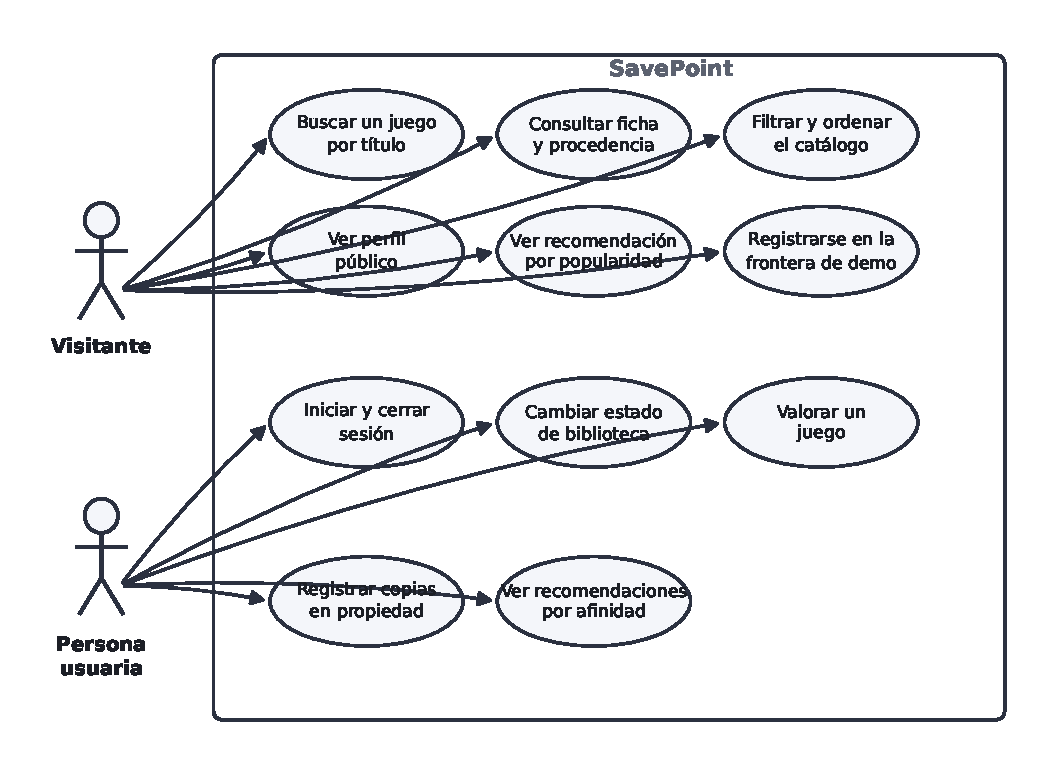
\includegraphics[width=0.95\textwidth]{figures/casos-uso.pdf}
    \caption{Diagrama de casos de uso del sistema, por actor principal. Cada línea une un actor con los casos de uso que ejecuta.}
    \label{fig:casos-uso}
\end{figure}

La Tabla~\ref{tab:casos-uso} describe cada caso de uso con su actor principal y el requisito
funcional que satisface.

\begin{table}[htp]
\centering
\begin{tabularx}{\textwidth}{ | C{0.10\textwidth} | Y | L{0.22\textwidth} | C{0.18\textwidth} | }
    \hline
    \textbf{Id} & \textbf{Caso de uso} & \textbf{Actor} & \textbf{Requisito} \\
    \hline
    CU-1 & Buscar un juego por título & Visitante & CAT-01 \\
    \hline
    CU-2 & Consultar la ficha de un juego y su procedencia & Visitante & CAT-03 \\
    \hline
    CU-3 & Filtrar y ordenar el catálogo & Visitante & CAT-02 \\
    \hline
    CU-4 & Ver la recomendación por popularidad & Visitante & REC-02 \\
    \hline
    CU-5 & Registrarse como persona usuaria & Visitante & AUTH-01 \\
    \hline
    CU-6 & Iniciar y cerrar sesión & Persona usuaria & AUTH-01 \\
    \hline
    CU-7 & Cambiar el estado de un juego en la lista de pendientes & Persona usuaria & LIB-01 \\
    \hline
    CU-8 & Valorar un juego & Persona usuaria & LIB-02 \\
    \hline
    CU-9 & Registrar una o varias copias en propiedad & Persona usuaria & INV-01, INV-02 \\
    \hline
    CU-10 & Abrir la página de recomendaciones por afinidad de géneros & Persona usuaria & REC-10 \\
    \hline
    CU-11 & Gestionar solicitudes de amistad, amistades y bloqueos & Persona usuaria & SOCIAL-03 \\
    \hline
    CU-12 & Consultar la colección de un amigo & Persona usuaria & SOCIAL-04 \\
    \hline
    CU-13 & Comentar un juego, con el comentario visible solo para los amigos & Persona usuaria & LIB-03, SOCIAL-04 \\
    \hline
    CU-14 & Editar el perfil y la privacidad de la cuenta & Persona usuaria & PROF-01 \\
    \hline
    CU-15 & Responder a una recomendación recibida de un amigo & Persona usuaria & SOCIAL-05 \\
    \hline
\end{tabularx}
\caption{Casos de uso del sistema.}
\label{tab:casos-uso}
\end{table}

\section{Requisitos de la evaluación de recomendadores}\label{sec:req-estudio}

La planificación posterior a la primera demostración añadió requisitos que no se pueden
validar únicamente recorriendo la interfaz. DATA-03 y DATA-06 exigen una frontera de corpus
gobernada, reversible y versionada, con checksum, diccionario, informe de calidad y muestra
determinista. DATA-05, DATA-07 y DATA-08 exigen importar valoraciones con procedencia, reconciliar
fuentes externas sin emparejamiento difuso y conservar una versión inmutable por cada versión del corpus.

EVAL-01, EVAL-02 y EVAL-03 fijan la comparación sobre la misma partición, los mismos
candidatos y las mismas exclusiones. EVAL-09 y EVAL-10 añaden usuarios sintéticos
parametrizados y obligan a separar la evidencia simulada de cualquier afirmación sobre
usuarios reales. DOC-04 exige que el protocolo, las métricas, las semillas, las versiones y
las amenazas a la validez queden escritos antes del resultado.

En recomendación, REC-01 exige un método de referencia aleatorio reproducible y REC-03 vectores de
contenido dispersos, perfil de usuario y similitud. REC-06 a REC-09 describen el arranque en frío,
las exclusiones, la explicación por contribuciones y el DTO versionado de las variantes
comparadas.

\begin{table}[H]
\centering
\tablecompact
\begin{tabularx}{\textwidth}{ | L{0.20\textwidth} | Y | L{0.20\textwidth} | }
    \hline
    \textbf{Área} & \textbf{Requisito de evaluación} & \textbf{Códigos} \\
    \hline
    Corpus & Frontera de corpus gobernada, reversible y versionada, con checksum, diccionario, informe de calidad y muestra determinista. & DATA-03, DATA-06 \\
    \hline
    Datos & Importación de valoraciones con procedencia, reconciliación sin emparejamiento difuso y conservación de una versión inmutable por corpus. & DATA-05, DATA-07, DATA-08 \\
    \hline
    Protocolo & Comparación sobre la misma partición, el mismo conjunto de candidatas y las mismas exclusiones. & EVAL-01, EVAL-02, EVAL-03 \\
    \hline
    Población & Usuarios sintéticos parametrizados y separación explícita entre evidencia simulada y conclusiones sobre usuarios reales. & EVAL-09, EVAL-10 \\
    \hline
    Documentación & Protocolo, métricas, semillas, versiones y amenazas a la validez fijados antes de conocer los resultados. & DOC-04 \\
    \hline
    Algoritmos & Método de referencia aleatorio reproducible. & REC-01 \\
    \hline
    Algoritmos & Vectores de contenido dispersos, perfil de usuario y similitud. & REC-03 \\
    \hline
    Algoritmos & Arranque en frío, exclusiones, explicación por contribuciones y DTO versionado de las variantes comparadas. & REC-06 a REC-09 \\
    \hline
\end{tabularx}
\caption{Requisitos de la evaluación de recomendadores.}
\label{tab:req-estudio}
\end{table}

\section{Requisitos no funcionales y reglas de negocio}\label{sec:req-no-funcionales}\label{sec:req-reglas}

Los requisitos no funcionales del sistema se agrupan en cinco familias. La
\textit{reproducibilidad} exige que el sistema arranque de forma reproducible en un entorno
local documentado, con las dependencias fijadas a versión exacta (QUAL-02, OPS-02). La
\textit{legalidad y procedencia de datos} exige que cada dato del catálogo conserve su
fuente, su licencia y su fecha de recuperación, con la elección de fuentes documentada junto
con sus términos (DATA-01, DATA-02, DATA-04, DATA-08). La \textit{accesibilidad y el diseño
responsive} exigen que los flujos principales funcionen con teclado y en anchuras de
escritorio y de móvil, verificables frente a las Pautas de Accesibilidad para el Contenido
Web (WCAG) 2.2 en nivel AA~\cite{wcag22} (QUAL-03). La \textit{seguridad} exige que ningún secreto aparezca en el control de versiones, en los paquetes del
navegador, en los registros ni en artefactos públicos. También exige que las acciones de
cambio de estado estén protegidas contra falsificación de petición en sitios cruzados
(SEC-02, SEC-04). La
\textit{calidad visual de producto} exige que la interfaz presente una densidad, una
tipografía y un tratamiento de la imagen propios de un producto de catalogación, no de un
prototipo utilitario (QUAL-05).

La Tabla~\ref{tab:reglas-negocio} recoge las reglas de negocio que gobiernan el
comportamiento del sistema.

\begin{table}[H]
\centering
\begin{tabularx}{\textwidth}{ | C{0.12\textwidth} | Y | }
    \hline
    \textbf{Regla} & \textbf{Enunciado} \\
    \hline
    RN-1 & La identidad de una obra es un identificador interno propio; el identificador del proveedor externo se guarda solo como procedencia. \\
    \hline
    RN-2 & El contenido descargable y las expansiones se muestran dentro de la página de su obra padre, nunca como resultado independiente del catálogo ni como entrada de biblioteca. \\
    \hline
    RN-3 & Los detalles privados de propiedad, como notas y datos de compra, nunca aparecen en ninguna proyección que vea otra persona. \\
    \hline
    RN-4 & La valoración se almacena como un entero de medias estrellas entre uno y diez; nunca como un número en coma flotante. \\
    \hline
    RN-5 & La recomendación por popularidad se calcula a partir de las señales de popularidad importadas de IGDB y nunca se presenta como personalizada. \\
    \hline
    RN-6 & La recomendación por afinidad de géneros refleja solo la actividad de la persona autenticada y nunca recurre a la recomendación de referencia por popularidad; sin historial suficiente, muestra un estado de bienvenida. \\
    \hline
    RN-7 & Registrar de nuevo una copia con la misma clave de idempotencia devuelve la copia existente en lugar de crear un duplicado. \\
    \hline
    RN-8 & Ninguna cuenta es pública: solo su titular y sus amigos aceptados acceden a su colección, sus listas y sus comentarios, y una persona sin sesión no ve ninguna cuenta. \\
    \hline
    RN-9 & El acceso a IGDB queda confinado a un comando de gestión fuera de línea; ninguna petición de usuario llama a un proveedor externo. \\
    \hline
    RN-10 & El nombre de usuario puede cambiarse una sola vez, y la visibilidad de la colección, los favoritos y las listas admite solo dos niveles: privada o visible para las amistades. \\
    \hline
\end{tabularx}
\caption{Reglas de negocio.}
\label{tab:reglas-negocio}
\end{table}

\section{Trazabilidad de requisitos}\label{sec:req-trazabilidad}

De los ochenta y ocho requisitos identificados en el análisis, ochenta y seis están
completos, con evidencia verificable en \texttt{docs/verification/} o en las firmas de
aceptación por fase. Entre ellos están las tres familias de recomendación y su protocolo de evaluación
sin conexión, que desarrollan la Sección~\ref{cap:algoritmos} y el Capítulo~\ref{cap:resultados}.
Los dos requisitos pendientes son parciales y pertenecen al mismo contrato de evaluación:
repetir la comparación de algoritmos con varias semillas y retroproyectar sobre la ejecución
v15 la captura de entorno y consumo de recursos. La Sección~\ref{sec:conc-limitaciones} los
recoge como limitaciones declaradas.

La Tabla~\ref{tab:trazabilidad-familias} recorre las dieciséis familias de requisitos del
proyecto, con cuántos de cada una están completos y verificados frente a los que quedan
pendientes. Cada fila es, en sí misma, una entrada de trazabilidad: el código de familia enlaza
directamente con los identificadores individuales de \texttt{.planning/REQUIREMENTS.md}; el
estado de cada uno de ellos remite a su vez a una firma de aceptación por fase o a un plan
concreto en \texttt{docs/verification/}.

\begin{table}[H]
\centering
\caption{Trazabilidad de requisitos de SavePoint, por familia.}\label{tab:trazabilidad-familias}
\tablecompact
\begin{tabularx}{\textwidth}{@{}>{\ttfamily\raggedright\arraybackslash}p{0.14\textwidth}Yrr@{}}
\textnormal{Familia} & \textnormal{Cubre} & \textnormal{Completos} & \textnormal{Total} \\
\hline
AUTH & Autenticación y sesión & 1 & 1 \\
PROF & Perfil personal & 3 & 3 \\
CAT & Catálogo, búsqueda y filtrado & 6 & 6 \\
LIB & Biblioteca y valoración & 4 & 4 \\
INV & Inventario de copias & 5 & 5 \\
DATA & Procedencia y gobierno de datos & 8 & 8 \\
REC & Algoritmos de recomendación & 10 & 10 \\
EVAL & Protocolo y laboratorio de evaluación & 10 & 12 \\
SEC & Seguridad & 8 & 8 \\
OPS & Operaciones y copia de seguridad & 5 & 5 \\
QUAL & Calidad de producto y accesibilidad & 5 & 5 \\
DOC & Documentación y registro & 6 & 6 \\
AGENT & Metodología de ingeniería & 6 & 6 \\
PORT & Portabilidad de datos & 4 & 4 \\
PRIV & Privacidad & 2 & 2 \\
SOCIAL & Relaciones sociales & 3 & 3 \\
\hline
\textbf{Total} & & \textbf{86} & \textbf{88} \\
\end{tabularx}
\end{table}

Los dos pendientes pertenecen a la familia \texttt{EVAL}; ningún requisito completo depende
de ellos para su propia verificación, de modo que ese trabajo futuro no invalida ninguna
evidencia ya cerrada.

La Tabla~\ref{tab:trazabilidad} enlaza cada requisito entregado con la evidencia que lo
respalda. La columna de evidencia remite a documentos del repositorio: firmas de aceptación
en \texttt{docs/verification/}, registros de decisión en \texttt{docs/adr/} e informes de
verificación en \texttt{.planning/phases/}.

\begin{table}[H]
\centering
\begin{tabularx}{\textwidth}{ | L{0.42\textwidth} | Y | }
    \hline
    \textbf{Requisito} & \textbf{Evidencia} \\
    \hline
    AUTH-01 & \texttt{phase-01-signoff.md}; pruebas de \texttt{accounts}. \\
    \hline
    CAT-01, CAT-03, CAT-04, CAT-06 & \texttt{phase-01-signoff.md}; \texttt{catalogue-freeze.md}. \\
    \hline
    LIB-01, LIB-02, INV-01, INV-02, INV-05 & \texttt{phase-01-signoff.md}; pruebas de \texttt{library}. \\
    \hline
    DATA-01, DATA-02 & \texttt{catalogue-freeze.md}; ADR-003. \\
    \hline
    REC-02 & \texttt{library/popularity.py}; \texttt{phase-01-signoff.md}. \\
    \hline
    SEC-02, OPS-01, OPS-02, OPS-03 & \texttt{phase-01-signoff.md}; \texttt{check-secrets.ps1}. \\
    \hline
    QUAL-03 & \texttt{phase-01-manual.md}; 400\% de zoom y lector de pantalla pendientes. \\
    \hline
    DOC-01, AGENT-01, AGENT-02, AGENT-03 & ADR-001 a 005; \texttt{agent-ledger.jsonl}. \\
    \hline
    DATA-04 & ADR-006; \texttt{igdb-api-probe.md}. \\
    \hline
    CAT-02 & \texttt{01.1-VERIFICATION.md} SC2; migración \texttt{0004}. \\
    \hline
    REC-10 & ADR-007; \texttt{01.1-VERIFICATION.md} SC5. \\
    \hline
    QUAL-05 & \texttt{phase-01.1-signoff.md}; revisión remota de capturas obtenidas durante la verificación. \\
    \hline
\end{tabularx}
\caption{Matriz de trazabilidad de requisito a evidencia.}
\label{tab:trazabilidad}
\end{table}

Este capítulo ha fijado qué debe hacer el sistema y con qué restricciones. El capítulo
siguiente describe cómo se ha diseñado para cumplirlo.
